\documentclass[11pt]{article}
\usepackage{fullpage}
\usepackage{setspace}
\usepackage{amsmath}
\usepackage{fancyvrb}
\usepackage{enumerate}
\usepackage{pgfplots}
\usepackage{graphicx}
\usepackage{float}
\usepackage{multirow}
\usepackage[format=hang,labelsep=quad]{caption}
\usepackage{subfig}
\usepackage{array}
\usepackage{multirow}


\begin{document}
\noindent\large{Math 5365}\\
\large{Data Mining 1}\\
\large{Homework 14}\\
\large{Mary Barker}
\doublespace
\begin{enumerate}
\item 
 Use gradient descent to minimize the function $f(x, y) = x^2 + y^2 + y$
 on the open disk $x^2 + y^2 < 1$. This is essentially the example on 
 p. 7 of the Lagrange multipliers slides, except that we are only 
 interested in interior points on this problem. 

 (Hints: Start by randomly selecting a vector (x, y) in the disk, and 
  then apply gradient descent. If the vector excapes the disk during the 
  algorithm, randomly select a new vector. Store vectors that converge 
  to a minimum in a matrix, and repeat the entire process a large number 
  of times to ensure that there is only one local minimum inside the disk. 
  You may need to take some care with the learning rate to prevent vectors 
  from escaping the disk too often.)

Using 300 initial guesses, the gradient descent function accurately computed 
the minimum point and gradient to within 10e-10 accuracy. 

\item
 Compare the merits of using a 2-layer neural network (with 1 hidden layer) 
 and a multi-layer neural network to the wdbc data set. Let's say you only 
 have 10 minutes to train a network with nnet or mlp. Which approach produces 
 the model with the higher classification accuracy? It may be interesting to 
 compare the two packages for a variety of time frames and to consider 
 different network topologies for mlp, e.g., size=c(2, 4) vs. size=c(2, 2, 2).

The first thing I considered was the effect of increasing the size of the hidden layer. 
The results, together with total time taken for each corresponding model are shown below. 
Note that the size of the data point corresponds to the length of time taken to 
produce the model. 

\begin{center}
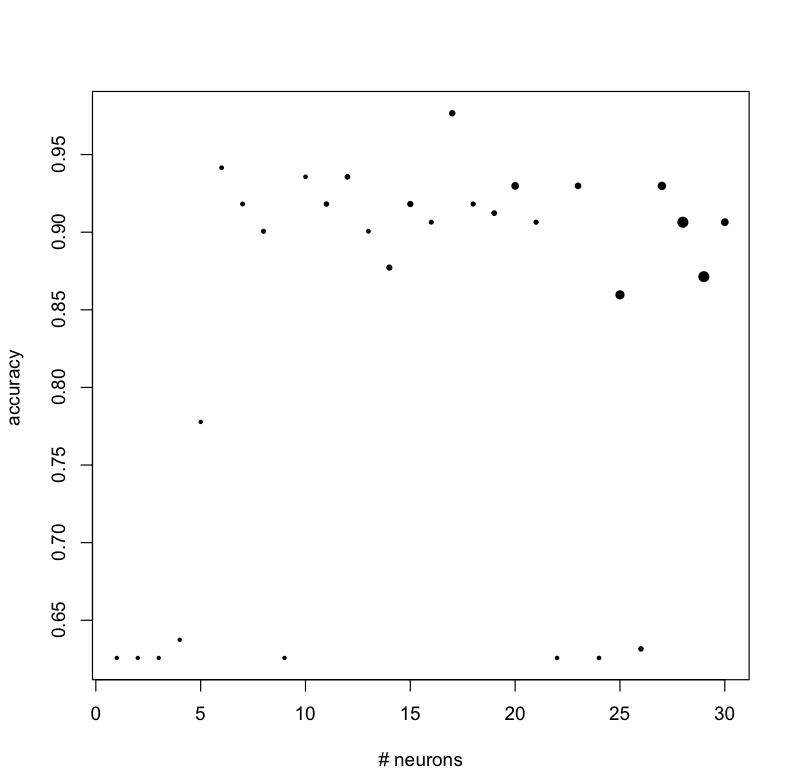
\includegraphics[scale=0.35]{pix/nnet_acc_size}
\end{center}

As can be seen, the overall runtime increases with the size of the hidden layer. 
However, the accuracy also increases dramatically between 1 and 5 neurons and then 
remains largely at the same level (with variation). The highest accuracy occured when 
using 17 neurons. With this model, the accuracy was approximately 98\%. The total time 
taken for this model is slightly above average at a value of 0.254 seconds 
where the maximum time taken was
0.799 seconds, the minimum time taken was 0.008, and the mean time was 0.1976 seconds.

For the multi-layer neural networks, I compared results using 2 through 5 hidden layers. 
In each case, the number of neurons in each layer was equal. Thus for a network with 
4 hidden layers and 16 total neurons, each layer contains 4 neurons. 

The results are shown in the graph below. As in the 
single hidden layer case above, the size of the point indicates the length of time taken 
to create the model. 

\begin{center}
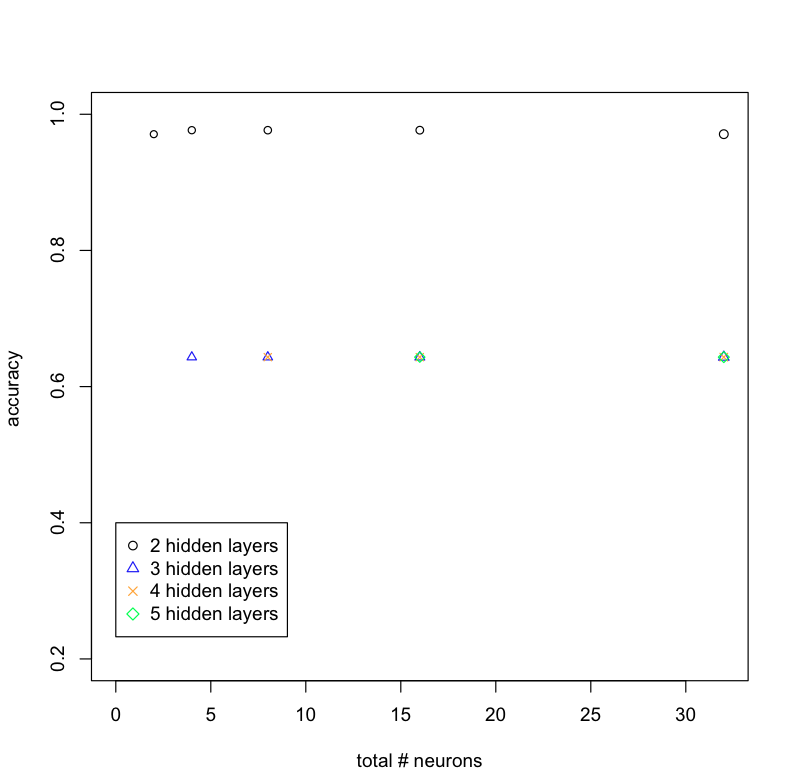
\includegraphics[scale=0.35]{pix/mlp_acc_size}
\end{center}

The average time taken was 0.8603333 seconds, with a minimum of 0.818 seconds using a 
neural network with 4 hidden layers and 1 neuron in each layer, and a maximum of 1.022 
seconds for a neural network with 2 hidden layers and 8 neurons in each layer. The 
variations in time with these cases are so small that time taken has little meaning 
except when compared with the case of a single hidden network. 

The maximum accuracy using multi-layer neural networks was roughly 98\%, the same 
as for 1 hidden layer. This level of accuracy was achieved using 4 neurons in each case.  

Thus it can be seen that for this problem, the most 
accurate models are not the most complex ones, but rather the single- and double-hidden layer 
models. In addition, the most time-efficient model is the single-layer model. Therefore the 
best model for this problem is a network with a single hidden layer and 4 neurons. 
\end{enumerate}

\begin{Verbatim}[numbers=left]

library(doMC)
registerDoMC()

source('~/Dropbox/Tarleton/data_mining/generic_functions/dataset_ops.R')

#1 Use gradient descent to minimize the function f(x, y) = x^2 + y^2 + y
#  on the open disk x^2 + y^2 < 1. This is essentially the example on 
#  p. 7 of the Lagrange multipliers slides, except that we are only 
#  interested in interior points on this problem. 

#  (Hints: Start by randomly selecting a vector (x, y) in the disk, and 
#   then apply gradient descent. If the vector excapes the disk during the 
#   algorithm, randomly select a new vector. Store vectors that converge 
#   to a minimum in a matrix, and repeat the entire process a large number 
#   of times to ensure that there is only one local minimum inside the disk. 
#   You may need to take some care with the learning rate to prevent vectors 
#   from escaping the disk too often.)

f <- function(x){
  return( sum(x^2) + x[2])
}

grad_f <- function(x){
   return(c(2*x[1], 2*x[2] + 1))
}

params <- function(x){
  if( sum(x^2) < 1){
  	return(TRUE)
  }else{
  	return(FALSE)
  }
}

initial_guess <- function(){
  x <- runif(2, -1, 1)
  return(x)
}

grad_descent <- function(f, grad_f, params, initial_guess, x0, eps, tol, niter){
  i = 1; NOT_ZERO = TRUE
  x = x0
  while((i < niter) && (NOT_ZERO)){
    i = i + 1
    xo = x
    x = xo - eps * grad_f(x)
    if(f(x) < f(xo)){
    	  eps = eps * 1.1
    }else{
    	  eps = eps * 0.5
    	}
    if(params(x)){
      if(abs(sum(grad_f(x)^2)) < tol){
        NOT_ZERO = FALSE
      }
    }else{
      x <- initial_guess()
      eps = 0.75 * eps
      i = 1
    }
  }
  return(list(grad = grad_f(x), x = x, dx = eps, 
              nit = i, converged = !NOT_ZERO))
}

######################################################################
# Initialize matrix of initial guesses and compute gradient descent  #
######################################################################
n_guesses = 300
x_m <- matrix(runif(n_guesses * 2, -1, 1), nrow = n_guesses, ncol = 2)
vals <- matrix(,nrow=n_guesses,ncol=2)

vals <- foreach(i=1:n_guesses, .combine=rbind) %dopar% {
  grad_descent(f, grad_f, params, initial_guess, x_m[i,], 0.9, 1.0e-17, 10000)$x
}

dx <- paste('TOTAL VARIATION IN COMPUTED CRITICAL POINT', 
            '\n variation in x-values -> ', 
            toString(max(vals[,1]) - min(vals[,1])),
            '\n','variation in y-values -> ',
             toString(max(vals[,2]) - min(vals[,2])))
writeLines(dx)
print(apply(vals, 1, grad_f))

#2 Compare the merits of using a 2-layer neural network (with 1 hidden layer) 
#  and a multi-layer neural network to the wdbc data set. Let's say you only 
#  have 10 minutes to train a network with nnet or mlp. Which approach produces 
#  the model with the higher classification accuracy? It may be interesting to 
#  compare the two packages for a variety of time frames and to consider 
#  different network topologies for mlp, e.g., size=c(2, 4) vs. size=c(2, 2, 2).

library(nnet)
library(RSNNS)

source('~/Dropbox/Tarleton/data_mining/class_notes/extras.R')
wdbc <- read.csv('~/Dropbox/Tarleton/data_mining/dfiles/wdbc.data', 
                  header=F, sep=',')
wdbc <- wdbc[,-1]
splitset <- splitdata(wdbc,0.7,F)
train <- splitset$train

## Consider first merely increasing size
len = 30


# 1   2     4      8        16
#    11     22     44       88 
#          1111   2222     4444
#               11111111 22222222
#                    1111111111111111

# accnnet <- rep(-1,len)
# for(i in 1:len){
  # model <- nnet(V2~., wdbc[train,], size=i,trace=F)
  # predvals <- predict(model,wdbc[-train,],type='class')
  # accnnet[i] <- confmatrix(wdbc$V2[-train], predvals)$accuracy
# }

normwdbc <- standardize(wdbc, 2:ncol(wdbc))
train_vals <- normwdbc[train,-1]
train_targ <- decodeClassLabels(normwdbc[train,1])
test_vals <- normwdbc[-train,-1]
test_targ <- decodeClassLabels(normwdbc[-train,1])

num = 4
accnnet <- rep(-1, num)
accmlpnet <- matrix(-1, num, num)
nnet_times <- rep(-1, num)
mlp_times <- matrix(-1, num, num)

for(i in 1:num){
  t_0 <- proc.time()
  model <- nnet(V2~., wdbc[train,], size=i, linout=F, trace=F)
  t_1 <- proc.time()
  nnet_times[i] <- t_1[3] - t_0[3]
  predvals <- predict(model, wdbc[-train,],type='class')
  accnnet[i] <- confmatrix(wdbc$V2[-train], predvals)$accuracy

  for(j in 1:num){
    if(j >= i){
      reps <- 2^(i - 1)
      vec <- rep(2^(j - i), reps)
      t_0 <- proc.time()
      model <- mlp(train_vals, 
                   train_targ, 
                   size=vec,  
                   maxit = 50, 
                   learnFuncParams = c(0.1),
                   inputsTest = test_vals,
                   targetsTest = test_targ,
                   linout = TRUE)
      t_1 <- proc.time()
      mlp_times[i,j] <- t_1[3] - t_0[3]
      idx <- (model$fittedTestValues[,1] >= 0.5) * 1
      predvals <- idx
      predvals[idx == 1] <- 'B'
      predvals[idx == 0] <- 'M'
      accmlpnet[i,j] <- confmatrix(wdbc$V2[-train], predvals)$accuracy
    }
  }
}
mlp_times
\end{Verbatim}
\end{document}
